% !TeX program = xelatex
\documentclass[pdflatex,iicol,sn-apa]{sn-jnl}
\usepackage{graphicx}
\usepackage{amsmath,amssymb}
\usepackage{booktabs,array,tabularx,multirow}
\usepackage{xcolor}
\definecolor{SeaBlue}{HTML}{5878A6}
\definecolor{SoftBlue}{HTML}{A7C7E7}
\definecolor{Coral}{HTML}{F4A7AE}
\definecolor{SeaTeal}{HTML}{A6D0C6}
\definecolor{PaleBlue}{HTML}{CFEAF6}
\definecolor{PalePeach}{HTML}{FBD9C9}
\definecolor{SoftGray}{HTML}{DADDE3}
\definecolor{DraftText}{HTML}{775326}
\newcommand{\pending}[1]{{\color{DraftText}\textit{[#1]}}}
\newcommand{\unmeasured}{\textcolor{DraftText}{TBD}}
\newcommand{\figureslot}[2]{\fcolorbox{SoftGray}{white}{\begin{minipage}[c][#1][c]{0.94\linewidth}\centering\small\color{SeaBlue}#2\end{minipage}}}
\newcolumntype{Y}{>{\raggedright\arraybackslash}X}
\AtBeginDocument{\renewenvironment{APACrefURL}{\par\noindent\url}{\par}}
\raggedbottom

\begin{document}

\title[Language-guided part segmentation]{Language-guided spatial prompting for part segmentation of generated 3D assets}
\author{\fnm{Author Information} \sur{Pending}}
\affil{\orgname{Affiliation Pending}}

\abstract{Part segmentation turns a generated three-dimensional (3D) asset into regions that can support inspection and editing. A single image can reveal the intended parts, yet class-agnostic masks often merge structures with similar appearance or divide one functional part into unrelated regions. We present a language-guided spatial prompting pipeline that constructs two-dimensional (2D) part guidance for a frozen 3D segmenter. A vision-language model (VLM) first identifies visible parts and predicts bounding boxes with positive and negative points. A prompted segmenter produces individual masks, which the VLM audits using overlays on the source image. Each rejected mask receives at most one prompt correction and segmentation retry. A deterministic assembly stage clips masks to the foreground, resolves overlaps with small-box priority, fills uncovered pixels, and assigns a fixed palette. The resulting guidance conditions SegviGen while its geometry and inference configuration remain shared across comparison conditions. Our evaluation separates guidance agreement, final-output projection agreement, and runtime reliability on an aligned collection of 500 assets. The assembled guidance raises 2D matched mIoU from 44.79\% to 51.53\% over automatic SAM2 regions, and the final-output projection improves from 34.19\% to 37.77\% on the 492 camera-aligned objects. Code is available at \pending{GitHub URL}.}

\keywords{3D Part Segmentation, Vision-Language Models, Spatial Prompting, Mask Refinement, Generated Assets}
\maketitle

\section{Introduction}
\label{sec:introduction}

Image-conditioned generation can produce textured 3D assets from a single observation. Compact structured representations have made this process applicable to objects with varied shapes and appearances \citep{xiang2025trellis2}. A generated surface, however, does not by itself identify the functional parts that a user might select, inspect, or edit. An outdoor air-conditioning unit contains a grille, service panel, and housing even when these surfaces share similar materials. Recovering such regions requires a decision about what constitutes a part as well as a decision about where its boundary lies. This distinction motivates part segmentation that can express semantic intent through explicit spatial evidence.

Recent methods learn 3D part features, support text queries, or predict masks directly from native 3D data \citep{ma2024find3d,liu2025partfield,ma2025p3sam,zhu2025partsam}. Another route transfers information from prompted 2D segmentation into a 3D representation \citep{cen2025sa3d,deng2025geosam2}. SegviGen further casts part segmentation as a structured coloring problem using a pretrained 3D generative prior \citep{li2026segvigen}. Its 2D-guided mode provides a useful interface for studying how a source-view partition affects the final 3D output. The quality of this interface depends on the supplied partition, including its part granularity, spatial support, and treatment of ambiguous regions.

Automatic image segmentation can produce visually plausible regions without identifying the parts required by a particular object. Similar appearance may cause a grille and surrounding panel to receive one mask. A different prompt may isolate a narrow frame but miss the larger component that it belongs to. Language can specify the intended component, but its name alone does not determine a precise pixel region. The useful intermediate representation therefore couples a part description to a box and point evidence. It must also accommodate the fact that the first spatial prediction may be wrong. In Fig.~\ref{fig:motivation}, the automatically produced guidance merges regions that are separated more clearly in the language-guided result and the designated reference.

\begin{figure*}[t]
\centering
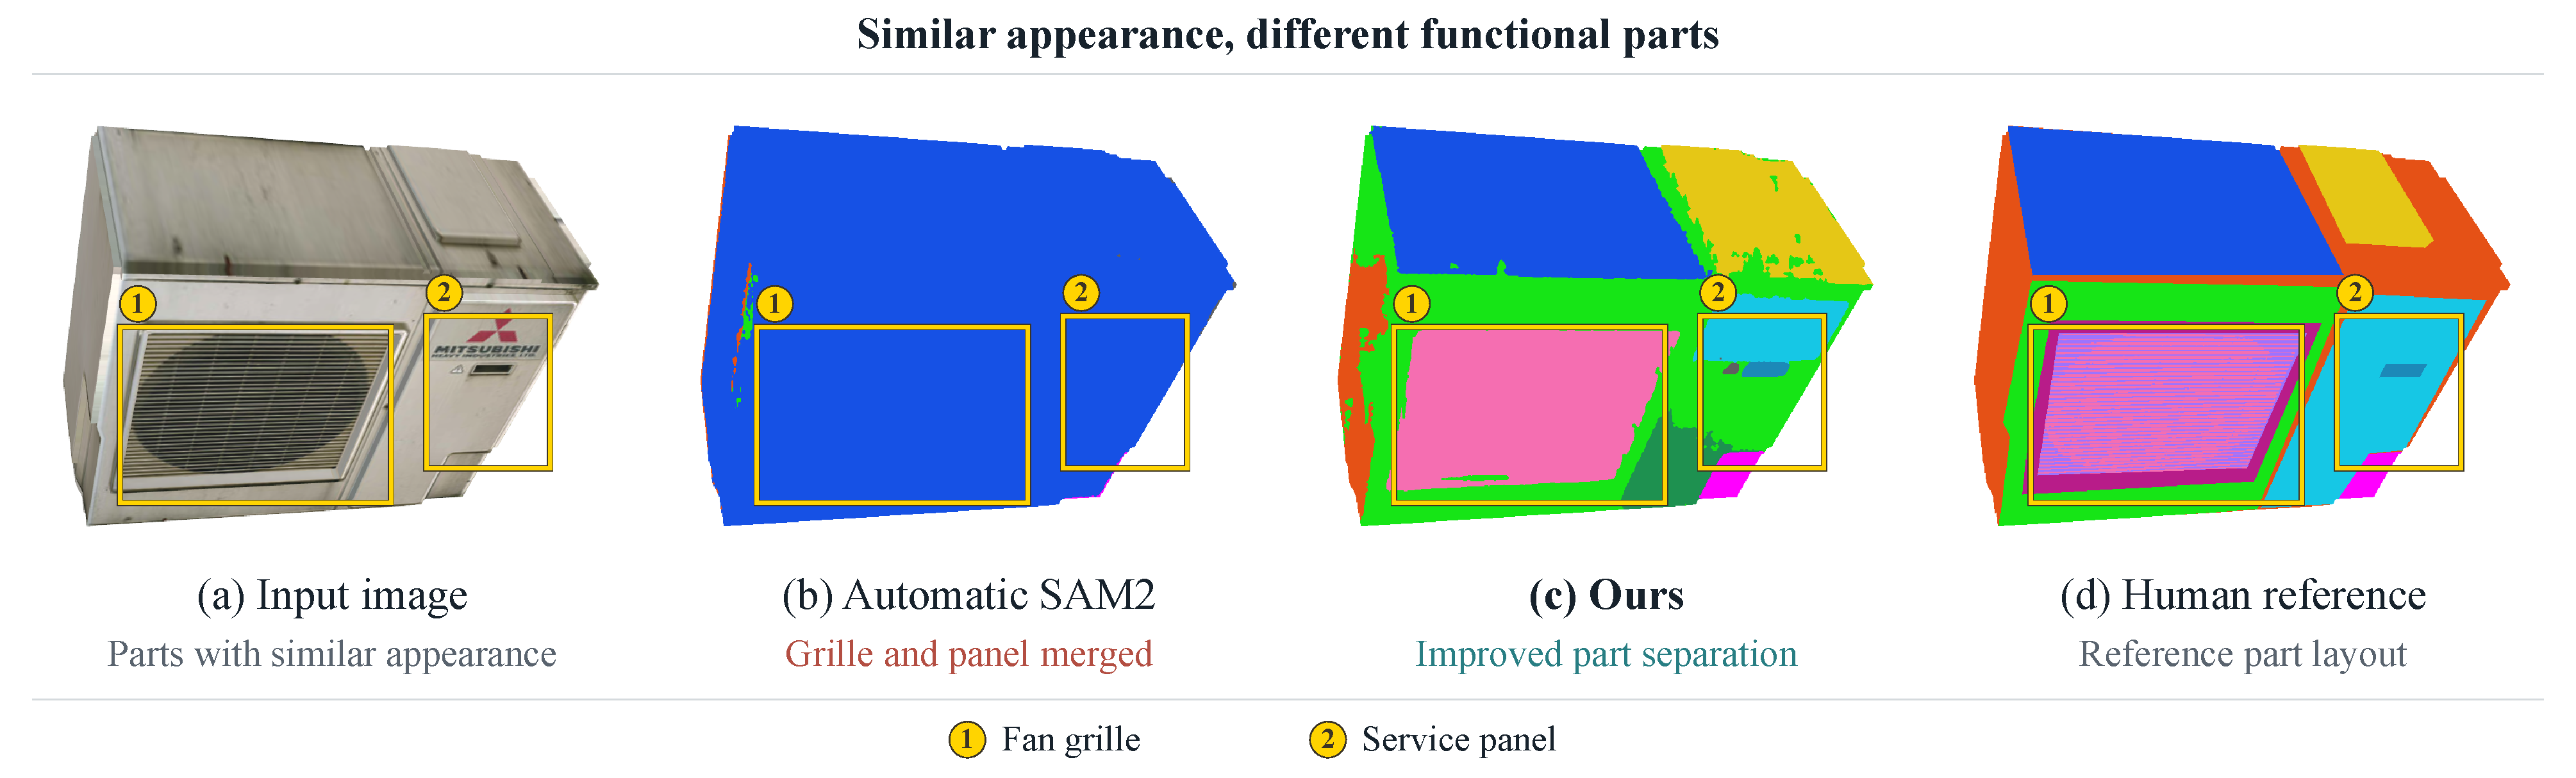
\includegraphics[width=\textwidth]{fig1_motivation.pdf}
\caption{Motivation using an outdoor air-conditioning unit from the aligned collection. The four panels show the source image, automatic SAM2 guidance, our guidance, and the designated human reference. Yellow boxes mark the fan grille and service panel. The example illustrates ambiguity between functional parts with similar appearance. Display colors are matched for comparison while the underlying region boundaries are retained. This is a source-view guidance example.}
\label{fig:motivation}
\end{figure*}

We construct guidance through part planning, individual-mask audit, and deterministic assembly. Qwen3-VL predicts names and spatial prompts from the source image \citep{bai2025qwen3vl}. SAM2 turns these prompts into masks \citep{ravi2024sam2}. The VLM then inspects each mask as a red overlay on the original appearance. A rejected mask receives refined spatial prompts and one segmentation retry. Auditing before assembly keeps each decision attached to a named candidate. Because palette colors carry no intrinsic semantics, the audit uses the original appearance and the candidate name. The accepted candidates are assembled into a foreground-complete guidance image by a reproducible sequence of operations.

The downstream 3D model is held fixed throughout this construction. The same image also supplies a shared reconstructed asset, which is normalized and voxelized for SegviGen. Only the guidance condition changes in the controlled A/B/C/D comparison. A is the original source image, B is automatic SAM2 guidance, C is the proposed pipeline, and D is the author-designated human reference condition. This comparison measures how changes in 2D guidance affect the final 3D partition under a shared geometry.

We connect language-based part identification to frozen 3D propagation through explicit spatial prompts, one correction per rejected mask, and deterministic foreground assembly. The associated evaluation distinguishes the quality of this partition from the behavior of the final 3D model, while keeping local part names in an explicit metadata record. The current aligned collection contains 500 objects across three structural groups. The evaluation protocol connects paired guidance comparisons to component ablations and computational measurements.

\section{Related work}
\label{sec:related}

\subsection{Part representations and 3D segmentation}
Learned representations provide several routes to 3D part understanding. Find3D learns features that can localize parts from open text queries \citep{ma2024find3d}. PartField learns continuous feature fields that support part clustering at different granularities \citep{liu2025partfield}. P3-SAM and PartSAM instead formulate promptable segmentation on native 3D data and include procedures for automatic decomposition \citep{ma2025p3sam,zhu2025partsam}. Hierarchical representations explicitly distinguish parts from their subparts \citep{gao2025latent}. These settings make granularity a central evaluation choice. Our setting specifies visible source-view parts before applying an existing 3D model, so the added mechanism acts at the guidance interface.

\subsection{Language and spatial evidence for parts}
Text can identify a functional part while visual evidence resolves its location. DM-PCL studies text-driven consistency for weakly supervised few-shot 2D part segmentation \citep{han2025dmpcl}. GMENet models object semantics, part relations, and boundaries through graph matching \citep{michieli2022gmenet}. Cross-model prior fusion provides another way to combine semantic and spatial representations \citep{zhao2026cmpf}. Our pipeline connects semantic and spatial evidence through explicit names, boxes, and points. Interactive feedback includes candidate selection through clicks \citep{jain2019click}, while reasoning video segmentation has also reused predicted masks as dense prompts \citep{dang2025decoupled}. Our audit instead operates on individual source-view part overlays and returns box-and-point corrections before deterministic assembly for a frozen 3D model.

\subsection{2D evidence and 3D propagation}
Radiance-field segmentation can propagate a prompted 2D mask through inverse rendering and cross-view self-prompting \citep{cen2025sa3d}. GeoSAM2 predicts masks on multiview geometric maps and aggregates them in 3D \citep{deng2025geosam2}. SegviGen uses a 3D generative prior and accepts a 2D part map as a condition for complete segmentation \citep{li2026segvigen}. We adopt this last interface and keep its parameters fixed. We construct and audit the input map while retaining the existing 3D propagation architecture. Evaluation-oriented studies also show the value of separating sources of segmentation difficulty through controlled comparisons \citep{yang2024benchmark}. This motivates reporting guidance, projection, structural-group, and reliability measurements separately.

\section{Method}
\label{sec:method}

\subsection{Overview and problem definition}
The input is a single red, green, blue, and alpha (RGBA) rendering $I$ of an object. The same rendering is used for 3D reconstruction and part planning. Let $I_{\mathrm{rgb}}$ denote its color channels and let $\alpha(x)$ denote its alpha value at pixel $x$. The foreground support is
\begin{equation}
F_{\alpha}=\{x\mid \alpha(x)>10\}.
\label{eq:foreground}
\end{equation}
At the source resolution, the method produces an integer label map $L$, a color guidance map $G$, and a metadata record $\mathcal A$. SegviGen combines $G$ with the shared voxel representation $V$ to produce a colored 3D partition. Figure~\ref{fig:pipeline} shows the complete data flow. The shaded 3D assets in this figure illustrate the interfaces between stages.

\begin{figure*}[t]
\centering
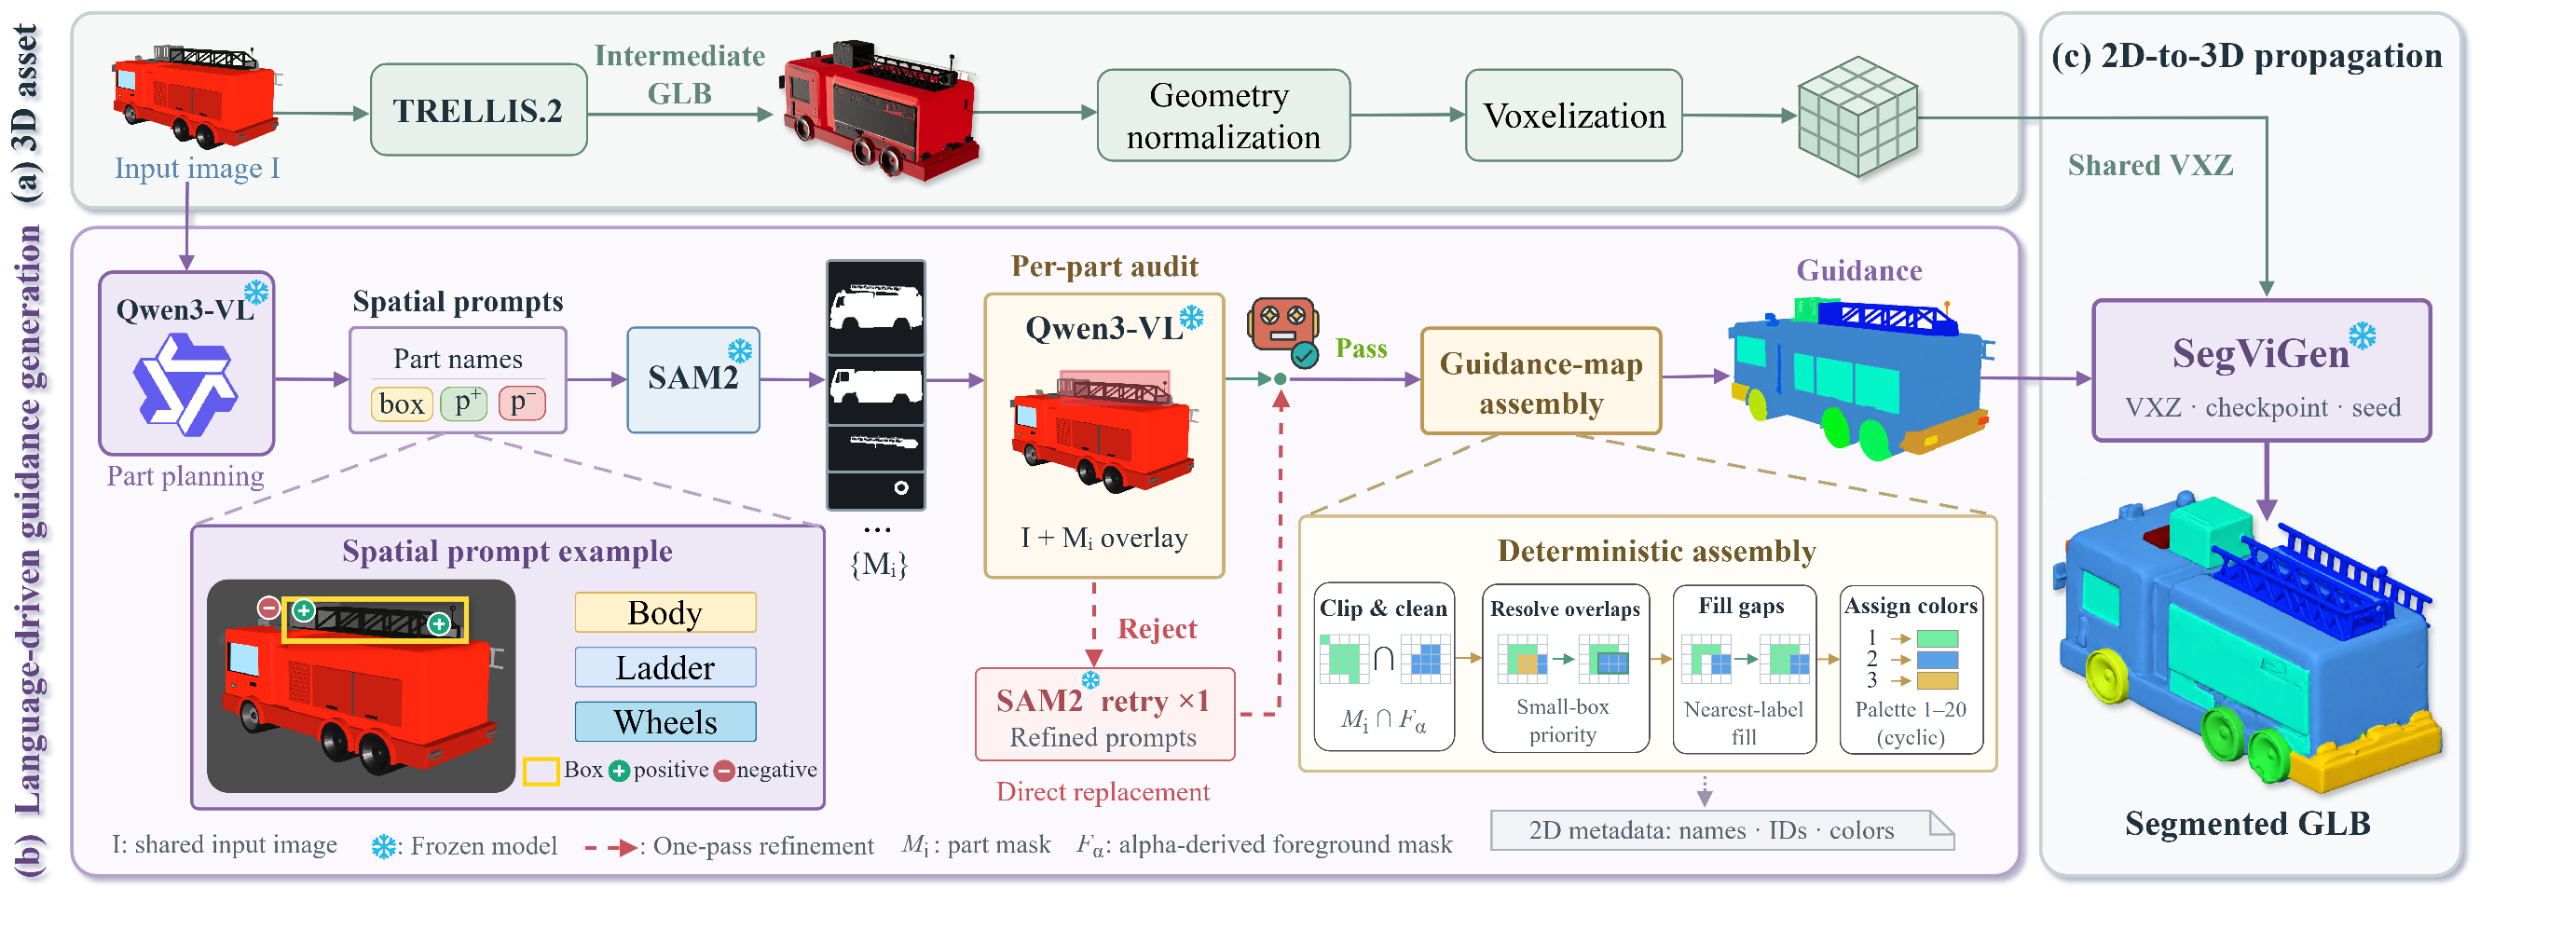
\includegraphics[width=\textwidth]{fig2_pipeline.pdf}
\caption{Main pipeline. The upper branch constructs a shared 3D asset from the input image through TRELLIS.2, an intermediate GLB, geometry normalization, and voxelization. The lower branch plans visible parts, predicts prompted masks, audits each candidate, and performs at most one SAM2 retry for a rejected candidate. Deterministic assembly comprises foreground clipping and cleaning, overlap resolution, gap filling, and palette assignment. The shared VXZ and assembled guidance enter frozen SegviGen. Names, local IDs, and colors are saved as 2D metadata. The diagrams of assets and masks are explanatory illustrations.}
\label{fig:pipeline}
\end{figure*}

The geometry branch supplies one common representation for all guidance conditions of an object. The guidance branch changes part assignments without regenerating that representation. This distinction is useful because the original downloaded model and the reconstructed model can have different topology and surface detail. The original asset provides the source rendering. The reconstructed geometry defines the object on which downstream segmentation is performed.

\subsection{Shared 3D asset construction}
TRELLIS.2 generates a textured mesh from $I$ \citep{xiang2025trellis2}. The exported binary glTF file, denoted by $\mathcal G$, is an intermediate representation. Geometry preprocessing applies the experiment's fixed normalization and coordinate convention before voxelization. We write this transformation as
\begin{equation}
V=\mathcal V\bigl(\mathcal N(\mathcal G)\bigr),
\label{eq:voxel}
\end{equation}
where $\mathcal N$ is the configured geometric preprocessing and $\mathcal V$ produces the sparse voxel asset stored as VXZ. SegviGen receives the resulting voxel representation together with the source-view guidance.

The collection uses upright source renderings whose image orientation is fixed before guidance generation. A/B/C/D runs reuse the same reconstructed mesh and VXZ of each object. Their segmentation checkpoint, sampling configuration, and random seed are also fixed. The output partitions can then be compared under the same 3D setup. The exact preprocessing transform and source camera remain part of the reproduction record, since a correct silhouette alone does not establish correspondence between source-view labels and rendered 3D surfaces.

\subsection{Visible part planning and spatial prompts}
Qwen3-VL receives $I_{\mathrm{rgb}}$ and proposes the visible components to be segmented \citep{bai2025qwen3vl}. Each candidate is represented by
\begin{equation}
r_i=(n_i,b_i,P_i^+,P_i^-),\qquad i=1,\ldots,K,
\label{eq:planning}
\end{equation}
where $n_i$ is the part name, $b_i$ is a bounding box, and $P_i^+$ and $P_i^-$ are positive and negative point sets. The proposal specifies a component visible in the given view. Repeated components can retain the same name while using different spatial records. This keeps semantic category and instance identity separate.

The box limits the search region. Positive points provide interior evidence, while negative points exclude nearby components that could otherwise be merged. The planner predicts coordinates in $[0,1000]$, which are converted to image coordinates using the actual width and height. Parsed values are clipped to valid image coordinates. Positive points are checked against the foreground and adjusted within the supported neighborhood when necessary. A proposal with no valid positive support is recorded and skipped. The part name remains associated with the record, but is not passed to SAM2 as a text prompt.

For every valid proposal, frozen SAM2 predicts a single candidate mask
\begin{equation}
M_i^{(0)}=S_{\theta}(I_{\mathrm{rgb}},b_i,P_i^+,P_i^-).
\label{eq:initialmask}
\end{equation}
All valid positive and negative points are used. SAM2 returns one mask per proposal. Its predicted quality score is retained when available and records the model's confidence, independently of the evaluation reference.

\subsection{Per-part audit and one-pass refinement}
The VLM inspects each initially valid mask before the masks are merged. Its input includes the source image, the candidate name, and an overlay that renders the mask in semitransparent red with a two-pixel contour. Retaining the source appearance makes it possible to inspect whether a predicted boundary follows the intended component. A black-and-white silhouette alone can hide the difference between a missing interior region and a correctly excluded neighboring surface. Each audit is attached to one candidate, so a rejected region can be traced back to its spatial prompt.

An accepted candidate retains $M_i^{(0)}$. A rejected candidate receives a corrected box when provided and additional positive or negative points. SAM2 is called once more with the resulting prompt
\begin{equation}
M_i^{(1)}=S_{\theta}\bigl(I_{\mathrm{rgb}},\widetilde b_i,
P_i^+\cup\Delta P_i^+,P_i^-\cup\Delta P_i^-\bigr).
\label{eq:refinement}
\end{equation}
When this retry produces a valid mask, it directly replaces the initial candidate. There is no second audit and no overlap-based choice between the old and new masks. If the audit cannot be parsed or the retry is invalid, the initial valid mask is retained and the event is recorded as partial. Each proposed part retains its audit outcome, and the number of segmenter calls remains bounded.

The refinement changes the prompt used for the retry. In the implementation used here, assembly still refers to the initial proposal's box and first valid positive point. These records define the overlap priority and component anchor below. Prompt correction therefore leaves the assembly order unchanged. Let $N\leq K$ be the number of proposals that enter the initial SAM2 call and let $K_v\leq N$ be the number producing valid initial masks. There are $N$ initial calls, $K_v$ audits, and at most $K_v$ retries. The total number of SAM2 calls is therefore at most $N+K_v\leq2N$. Retry counts are measured as part of runtime analysis.

\subsection{Deterministic guidance-map assembly}
Individual masks can overlap, contain disconnected spill regions, or leave foreground pixels uncovered. Assembly turns them into one complete partition without asking the VLM to select RGB values. Its four operations follow the expanded panel in Fig.~\ref{fig:pipeline}. A semantic proposal remains a distinct integer label through these operations. Palette colors are introduced only after the partition has been resolved.

\subsubsection{Clip and clean}
Let $M_i$ denote the mask selected by the audit procedure and let $p_i$ denote the first valid positive point of the initial proposal. The cleaned candidate is
\begin{equation}
\overline M_i=\mathcal C(M_i\cap F_{\alpha},p_i).
\label{eq:clean}
\end{equation}
The cleaning operator first uses eight-connected components. The component supported by $p_i$ is retained as the main component. If the point falls outside the predicted region, the nearest component is used. Without an available anchor, the largest component is selected. Additional components with area at least $\max(96,\lfloor0.18a_i\rfloor)$ are retained, where $a_i$ is the main component's area. This allows a part to have separated visible fragments while suppressing small spill regions.

The mask then undergoes closing with a $3\times3$ elliptical element, another foreground clip, and component filtering. Small enclosed holes are filled if their area is at most $\max(48,\lfloor0.00015|F_{\alpha}|\rfloor)$. Background regions connected to the image boundary are not filled as holes. A cleaned candidate must meet the area threshold $\max(a_{\min},96,\lfloor0.00012|F_{\alpha}|\rfloor)$, where $a_{\min}$ is the configured minimum. The default implementation uses $a_{\min}=10$ at the source resolution. These are resolution-dependent image operations.

\subsubsection{Resolve overlaps}
Large masks can contain a smaller component together with the surrounding housing. If the larger mask claims the overlap first, the smaller component may have no pixels left. Assembly therefore sorts candidates by increasing initial box area. Cleaned mask area and candidate ID break ties deterministically. With order $\pi$ and initially empty occupied set $U_0$, the remaining region of the next candidate is
\begin{equation}
R_{\pi(t)}=\overline M_{\pi(t)}\setminus U_{t-1}.
\label{eq:overlap}
\end{equation}
The region is accepted if it has at least $\max(a_{\min},96,\lfloor0.00010|F_{\alpha}|\rfloor)$ pixels. Its pixels receive a new local ID and are added to $U_{t-1}$. Otherwise the candidate is dropped with an explicit reason. Box area determines priority independently of the part name and the evaluation reference. The ablation tests the effect of this ownership rule.

\subsubsection{Fill gaps}
Let $U$ be the union of accepted regions. Every unassigned foreground pixel is given the label of its nearest accepted pixel
\begin{equation}
L(x)=L\!\left(\arg\min_{y\in U}\|x-y\|_2\right),
\qquad x\in F_{\alpha}\setminus U.
\label{eq:gaps}
\end{equation}
A Euclidean distance transform implements this assignment. Existing labeled pixels retain their ownership and background pixels remain zero. Gap filling completes the support of the predicted partition using already accepted parts. It does not add another semantic proposal. If no candidate survives, the procedure records a failure.

\subsubsection{Assign colors}
The integer map is saved before palette conversion. With palette $c_0,\ldots,c_{20}$ and background index zero, the guidance color is
\begin{equation}
G(x)=
\begin{cases}
c_0,&L(x)=0,\\
c_{1+((L(x)-1)\bmod20)},&L(x)>0.
\end{cases}
\label{eq:palette}
\end{equation}
The script assigns colors deterministically. The VLM neither chooses palette indices nor edits the assembled image. The 20 foreground colors are reused cyclically when there are more than 20 labels. A 16-bit label image therefore remains the identity-bearing representation, since a reused RGB value can represent multiple local IDs. The metadata stores the retained name, local ID, palette index, and associated mask. These records describe the 2D partition.

\subsection{Frozen 3D propagation}
The downstream interface is summarized by
\begin{equation}
\widehat{\mathcal G}_k=H_{\phi}(V,G_k;\xi),
\qquad k\in\{A,B,C,D\},
\label{eq:downstream}
\end{equation}
where $\phi$ denotes the frozen SegviGen checkpoint and $\xi$ its sampling configuration. In the A condition, $G_A$ is the source image rather than an explicit part map. B uses automatic SAM2 guidance, C uses our assembled guidance, and D uses the designated human reference map. SegviGen extracts the image condition, samples its structured texture representation, and exports the colored result. These internal stages are kept abstract in our method figure because the contribution lies in constructing the upstream condition.

Names are retained in the separate 2D metadata and are not supplied to the 3D model as text. Likewise, a color in the exported GLB is not by itself a persistent semantic surface ID. Evaluating or editing such an ID requires an explicit surface-to-label correspondence. We evaluate the colored partitions through the label and projection protocols defined below. The 2D metadata does not establish a semantic correspondence to individual 3D surfaces.

\section{Experiments}
\label{sec:experiments}

\subsection{Data and evaluation sets}
The assets originate from Objaverse \citep{deitke2023objaverse}. The current aligned manifest contains 500 unique objects, comprising 154 assemblies, 181 solid-volume objects, and 165 thin or fine-grained objects. These structural groups support analysis of connected subassemblies, broad regions, and narrow structures. They are experimental strata rather than semantic object classes. Each retained object has A/B/C/D outputs and references to the shared source image and geometry. Asset completeness is checked independently of segmentation quality.

The aligned subset was selected using availability and C-run success conditions. It supports paired output-quality comparisons conditional on that selection. Runtime failure rates must instead use the prespecified attempted population before this filtering. The full attempt manifest, exclusions, and counts for each method will be attached to the final evaluation. Objects used to adjust prompts or inspect intermediate failures must be identified separately from a held-out test set. \pending{Finalize the development/test split and the original attempted-population denominator.}

D denotes the designated standard reference: a human-repaired source-view part map specified by the authors as the evaluation reference. Part IDs are local to an object. The stored mapping records annotation provenance and verification status, which are retained during evaluation. \pending{Complete and report the reference audit, ignored regions, annotation protocol, and inter-annotator checks.} The source-view reference specifies visible regions. It is not a fully labeled 3D mesh, and the original unsegmented Objaverse asset is not used as a part reference. The D labels are the scoring reference for both guidance and projection metrics; the D-guided 3D output itself enters only as an additional input condition that marks the level reached when the reference map is used as guidance.

\subsection{Implementation and controlled conditions}
The implementation uses Qwen3-VL for planning and mask audit, with SAM2 for prompt-conditioned mask prediction. The source images and guidance maps are $1024\times1024$. The available five-object configuration uses Qwen3-VL-4B-Instruct and SAM2.1 Hiera base-plus. \pending{Confirm the model identifiers and frozen configuration for the full C run.} All pretrained components remain frozen. The same prompt parsing, source-image orientation, and alpha support are used throughout an object's guidance construction.

The recorded 3D configuration uses voxel resolution 512, the \texttt{full\_seg\_w\_2d\_map.ckpt} checkpoint, 20 sampling steps, and seed 42. The export configuration enables remeshing with a target of 100,000 faces and a texture size of 4096. The shared geometry and sampling configuration are common to A/B/C/D for each retained object. The manifest links each guidance condition to its actual input geometry and inference configuration.

\subsection{Comparison methods}
The external comparison includes Find3D, PartField, P3-SAM, GeoSAM2, and SegviGen \citep{ma2024find3d,liu2025partfield,ma2025p3sam,deng2025geosam2,li2026segvigen}. All are evaluated on the same reconstructed assets under an explicit input protocol. Find3D requires a fixed procedure for obtaining part text queries. PartField requires a fixed clustering and granularity setting. P3-SAM uses its automatic decomposition setting for automatic comparisons. Reference part counts are not used to select a favorable output granularity for an individual test object.

GeoSAM2 uses spatial prompts and multiview geometric maps. A shared-prompt adaptation must specify how the source-view guidance is converted into its supported interface and whether extra views are rendered. The original SegviGen comparison must identify its complete-segmentation condition separately from the controlled A/B/C/D experiment. The input-condition column in Table~\ref{tab:main} records these differences. Published benchmark numbers are not transferred into the cells for our collection. \pending{Freeze each external method's automatic or prompted configuration before running the comparison.}

\subsection{Guidance and projection metrics}
Predicted integer labels are compared with reference regions after excluding predefined ignored pixels. Background is excluded from the part list, while predicted leakage into reference background remains in the region union. For predicted parts $P_1,\ldots,P_m$ and reference parts $D_1,\ldots,D_n$, intersection over union (IoU) is
\begin{equation}
J_{ij}=\frac{|P_i\cap D_j|}{|P_i\cup D_j|}.
\label{eq:iou}
\end{equation}
Local integer IDs and display RGB values need not agree across methods. Region correspondence is determined by overlap, rather than by assuming a common palette identity.

Matched mean IoU (mIoU) uses a one-to-one assignment that maximizes the sum of pairwise overlaps
\begin{equation}
\operatorname{mIoU}_{\rm match}
=\frac{1}{n}\max_{\pi}\sum_{j\in\operatorname{dom}(\pi)}J_{\pi(j),j}.
\label{eq:matched}
\end{equation}
Here $\pi$ is a partial injection from reference to predicted parts. Unmatched reference regions contribute zero through the fixed denominator $n$. Additional predictions are assessed by part F1 at IoU threshold 0.5. Its matching maximizes the number of pairs that meet the threshold, and with $T$ matched pairs the score is $2T/(m+n)$. This objective differs from maximizing the IoU sum. The two scores jointly expose missed and excessive partitions.

Boundary F1 (BF1) is measured on the nonzero-overlap pairs of the IoU assignment using a two-pixel boundary tolerance at the fixed source resolution. The per-pair values are averaged over the reference part count, assigning zero to unmatched reference regions. Ignored areas are removed with the corresponding boundary treatment. The object is the aggregation unit. Guidance and controlled A/B/C/D summaries use the reported structural-group macro-averages. The updated P3-SAM, GeoSAM2, and PartField results in Table~\ref{tab:main} instead give each of the 500 objects equal weight.

For final-output evaluation, each segmented GLB is projected from the fixed source camera to a discrete label map, using label rendering that does not introduce illumination-dependent colors. The projected regions are scored with the same matching and boundary rules. The scored label map is rendered from the final 3D output. Camera transforms, orientation, and silhouette alignment are checked before a sample contributes a score. Source-view projection measures agreement on the visible surface. Multiview qualitative assessment addresses additional views, while full 3D IoU would require a separately labeled 3D reference.

\subsection{Main comparison}
Table~\ref{tab:main} reports final-output projection mIoU, boundary F1, and the available Part F1 measurements. P3-SAM, GeoSAM2, and PartField use object-weighted means over 500 objects. The other rows retain their recorded coverage and aggregation. The paired A/B/C/D comparison below measures the effect of guidance on the shared camera-aligned set.

\begin{table*}[t]
\caption{Final-output projection results against the designated source-view reference at $1024\times1024$, with a two-pixel boundary tolerance and Part F1 at IoU 0.5. PartField, P3-SAM, and GeoSAM2 use the updated object-weighted summaries over 500 objects. Find3D retains its 468-object summary. SegviGen and Ours retain the 492-object camera-aligned summaries (contour IoU $\geq0.50$). Sample coverage and aggregation differ across these rows; the controlled A/B/C/D comparison in Table~\ref{tab:controlled} uses a shared evaluation set. Unavailable Part F1 values are marked TBD.}
\label{tab:main}
\centering\small
\setlength{\tabcolsep}{4pt}
\begin{tabularx}{\textwidth}{@{}Y >{\raggedright\arraybackslash}p{2.9cm} c c c c@{}}
\toprule
Method & Part condition & \shortstack{Proj. mIoU\\(\%) $\uparrow$} & \shortstack{Boundary F1\\(\%) $\uparrow$} & \shortstack{Part F1@0.5\\(\%) $\uparrow$} & \shortstack{Evaluable\\$N$}\\
\midrule
Find3D \citep{ma2024find3d} & Text queries & 30.66 & 26.38 & \unmeasured & 468\\
PartField \citep{liu2025partfield} & Feature clustering ($K{=}10$) & 32.71 & 13.94 & 16.75 & 500\\
P3-SAM \citep{ma2025p3sam} & Automatic & 38.19 & 17.92 & 35.13 & 500\\
GeoSAM2 \citep{deng2025geosam2} & Shared prompts & 24.35 & 10.88 & 31.66 & 500\\
SegviGen \citep{li2026segvigen} & No part prompt & 34.19 & 31.45 & \unmeasured & 492\\
Ours & 2D guidance & 37.77 & 35.29 & \unmeasured & 492\\
\bottomrule
\end{tabularx}
\end{table*}

\begin{table*}[t]
\caption{Controlled guidance comparison under shared geometry and frozen SegviGen settings. The 2D columns score each guidance map itself against the designated standard reference on the 500 paired objects; A supplies the raw source image and has no explicit part map, and the D guidance is the reference map itself. The projection columns score the final 3D output on the 492 camera-aligned objects. The B row exposes the 2D ambiguity that motivates the pipeline: automatic regions merge or split functional parts. The 2D gain from B to C survives propagation, while the D row marks the reference-guidance ceiling.}
\label{tab:controlled}
\centering\small
\setlength{\tabcolsep}{5pt}
\begin{tabularx}{\textwidth}{@{}Y >{\raggedright\arraybackslash}p{4.2cm} c c c c@{}}
\toprule
Condition & Guidance Input & \shortstack{2D mIoU\\(\%) $\uparrow$} & \shortstack{2D BF1\\(\%) $\uparrow$} & \shortstack{Proj. mIoU\\(\%) $\uparrow$} & \shortstack{Proj. BF1\\(\%) $\uparrow$}\\
\midrule
A & Source image (no part map) & --- & --- & 34.19 & 31.45\\
B & Automatic SAM2 regions & 44.79 & 44.74 & 35.77 & 32.41\\
C & Ours (assembled guidance) & 51.53 & 46.87 & 37.77 & 35.29\\
D & Reference map (ceiling) & --- & --- & 50.97 & 47.52\\
\bottomrule
\end{tabularx}
\end{table*}

The controlled guidance comparison uses A/B/C/D with common geometry and SegviGen settings (Table~\ref{tab:controlled}). A tests the original appearance as a condition, while B supplies automatic regions. C replaces those regions with the proposed language-guided partition. D measures the output obtained from the designated-standard-reference guidance condition. The 6.74-point 2D gain from B to C survives frozen 3D propagation as a 2.00-point projection gain, and the paired C--A projection gap is 3.58 points. The D condition reaches 50.97\% projection mIoU, and the C--D gap shows that the frozen backend can produce better projection agreement when given the reference partition.

Figure~\ref{fig:guidance} compares the author-provided 2D guidance examples across the four conditions. The examples include assemblies, solid-volume objects, and thin or fine-grained structures. The traffic-cone example has identical automatic and reference masks, illustrating why the number of predicted regions alone does not establish agreement with a reference partition. These images show the input conditions before 3D inference. Figure~\ref{fig:qualitative} shows six selected examples rendered from the final A/B/C/D GLB outputs. The four conditions in each row share a display view, scale convention, and lighting. C separates the traffic cone from its base and distinguishes the chair backrest from the seat, whereas B largely merges these structures. Separation remains incomplete: the cone retains a small extra region at its rim, and several chair legs still merge with the seat. These selected views illustrate output behavior; the quantitative results use the fixed scoring cameras.

\begin{figure*}[t]
\centering
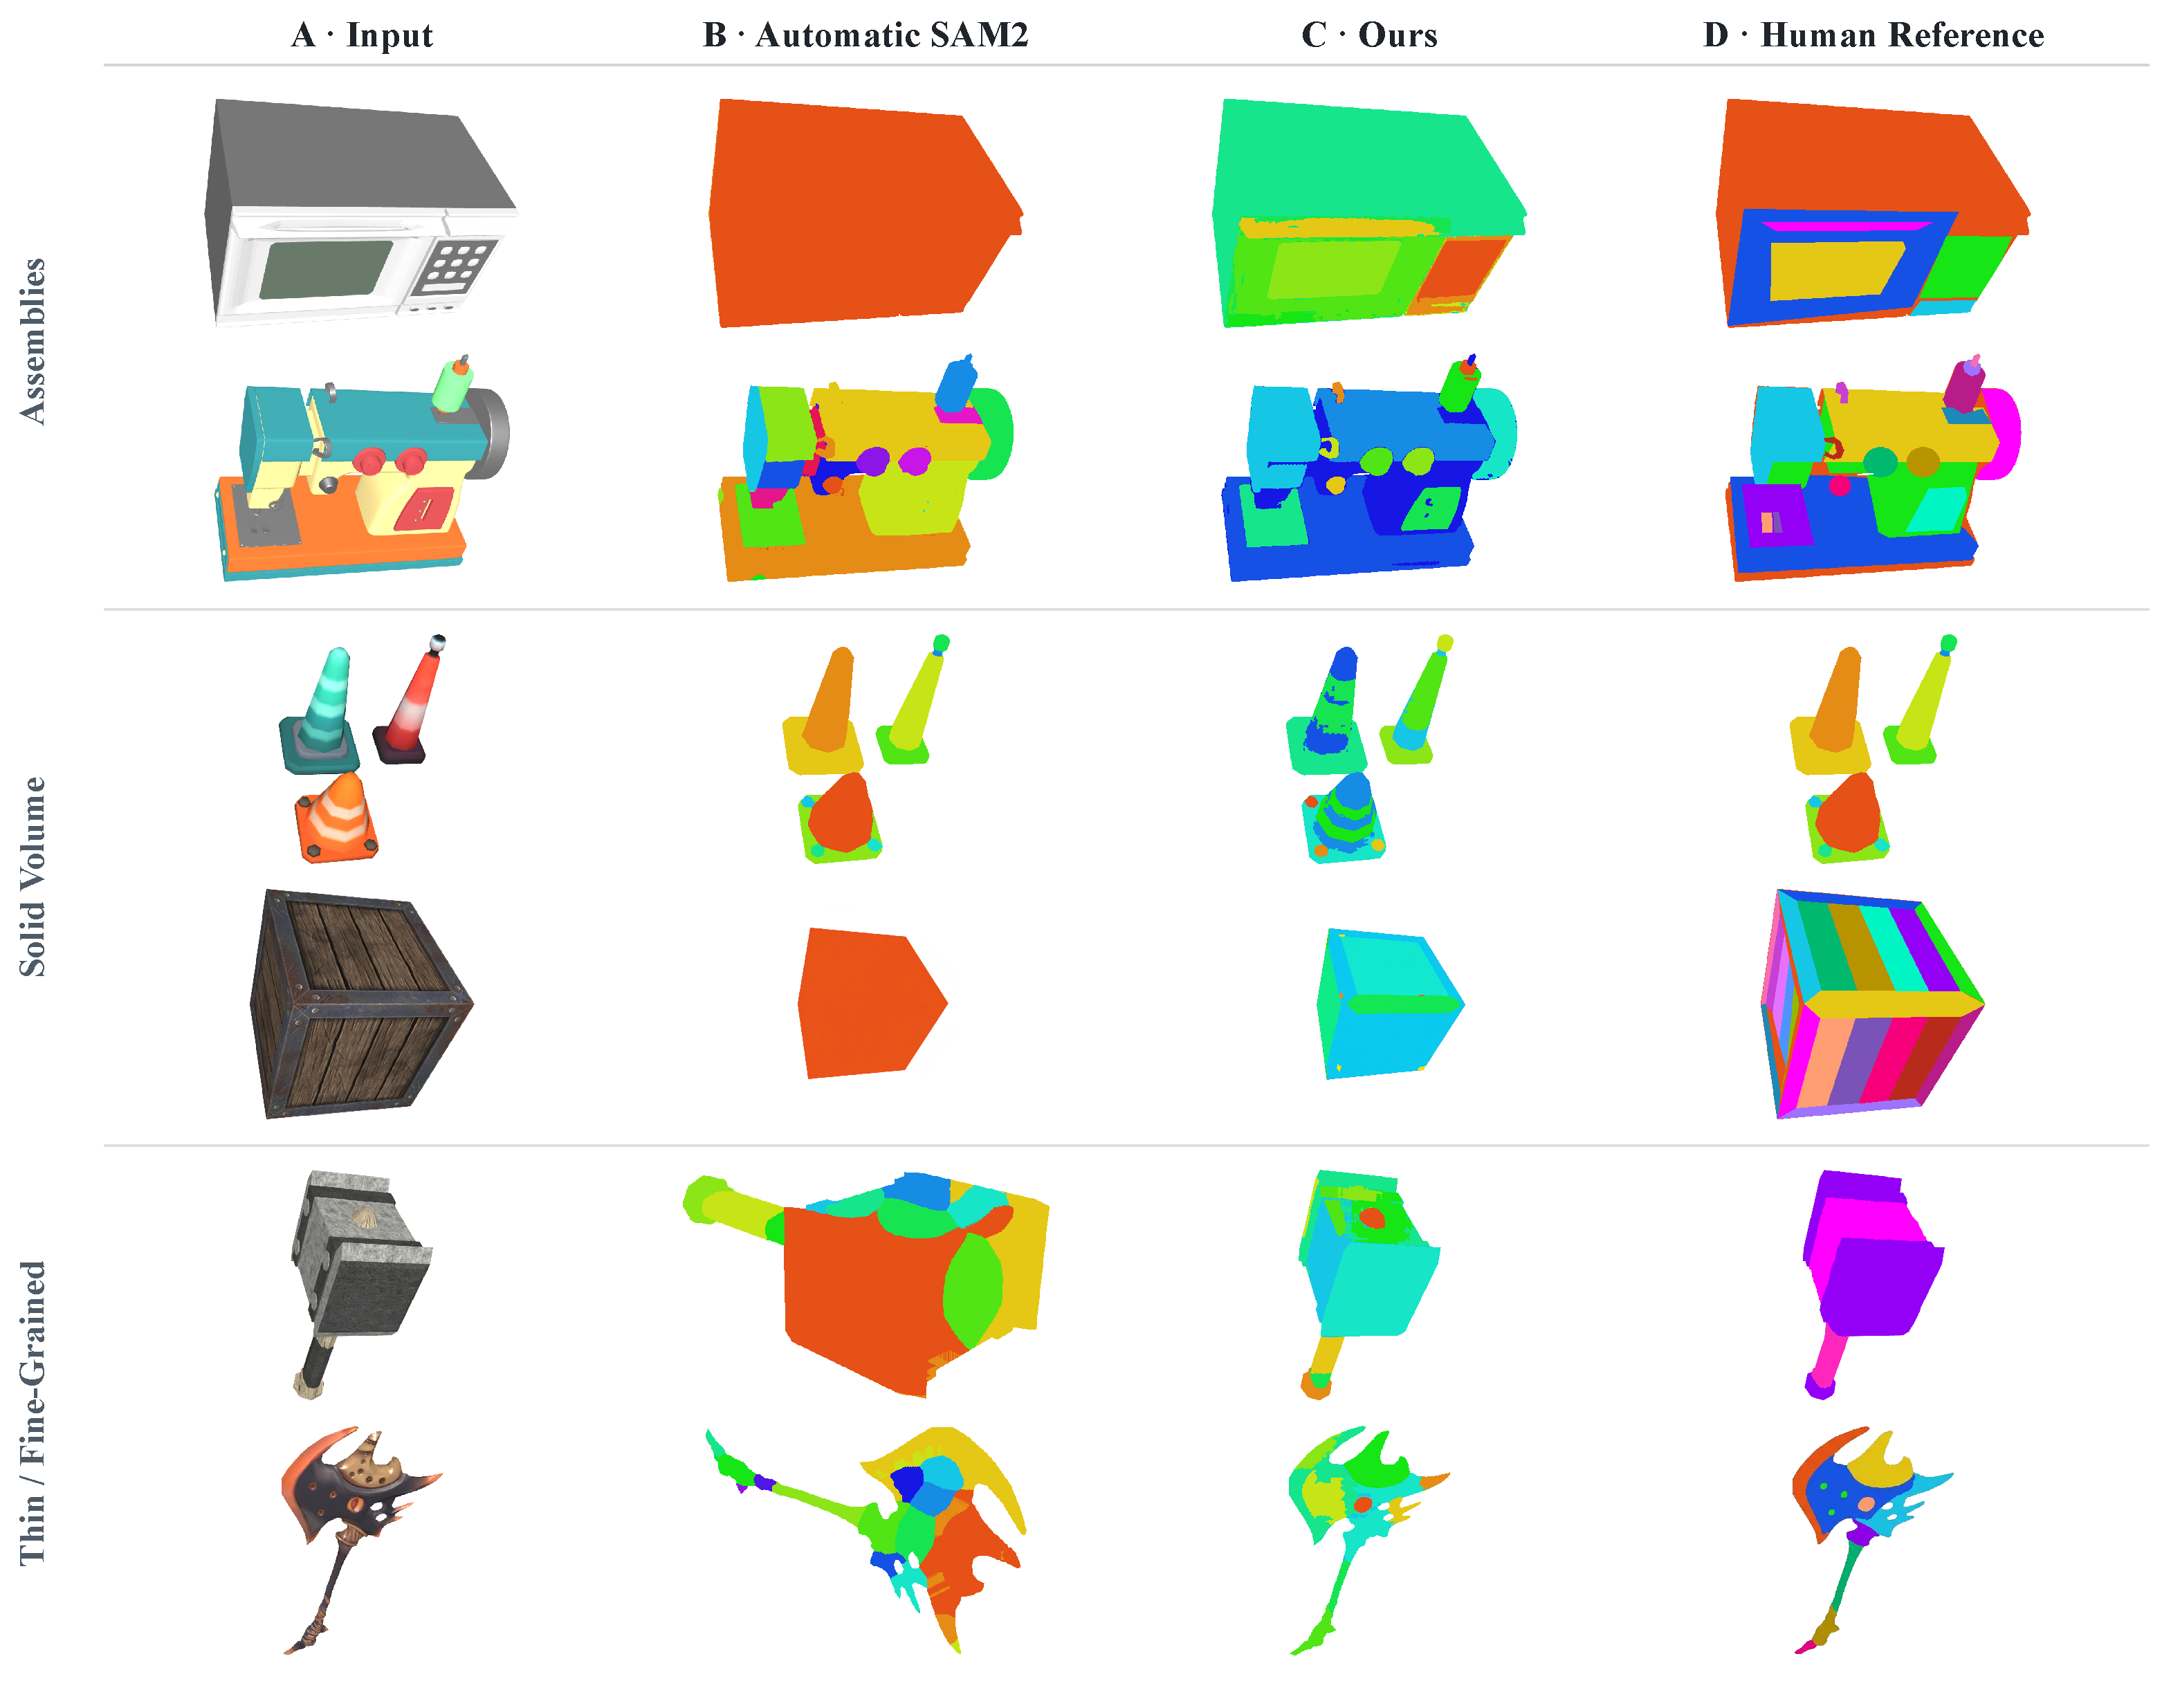
\includegraphics[width=\textwidth]{fig3_guidance.pdf}
\caption{2D guidance comparison using the supplied visualization examples. Columns show the input image, automatic SAM2 guidance, our guidance, and the designated human reference. Rows are grouped into assemblies, solid-volume objects, and thin or fine-grained structures. Colors identify local regions and do not imply shared part IDs across conditions. The automatic and reference traffic-cone masks are identical in the supplied data. \pending{Align the B-column orientation for the hammer and axe before final publication.}}
\label{fig:guidance}
\end{figure*}

\begin{figure*}[t]
\centering
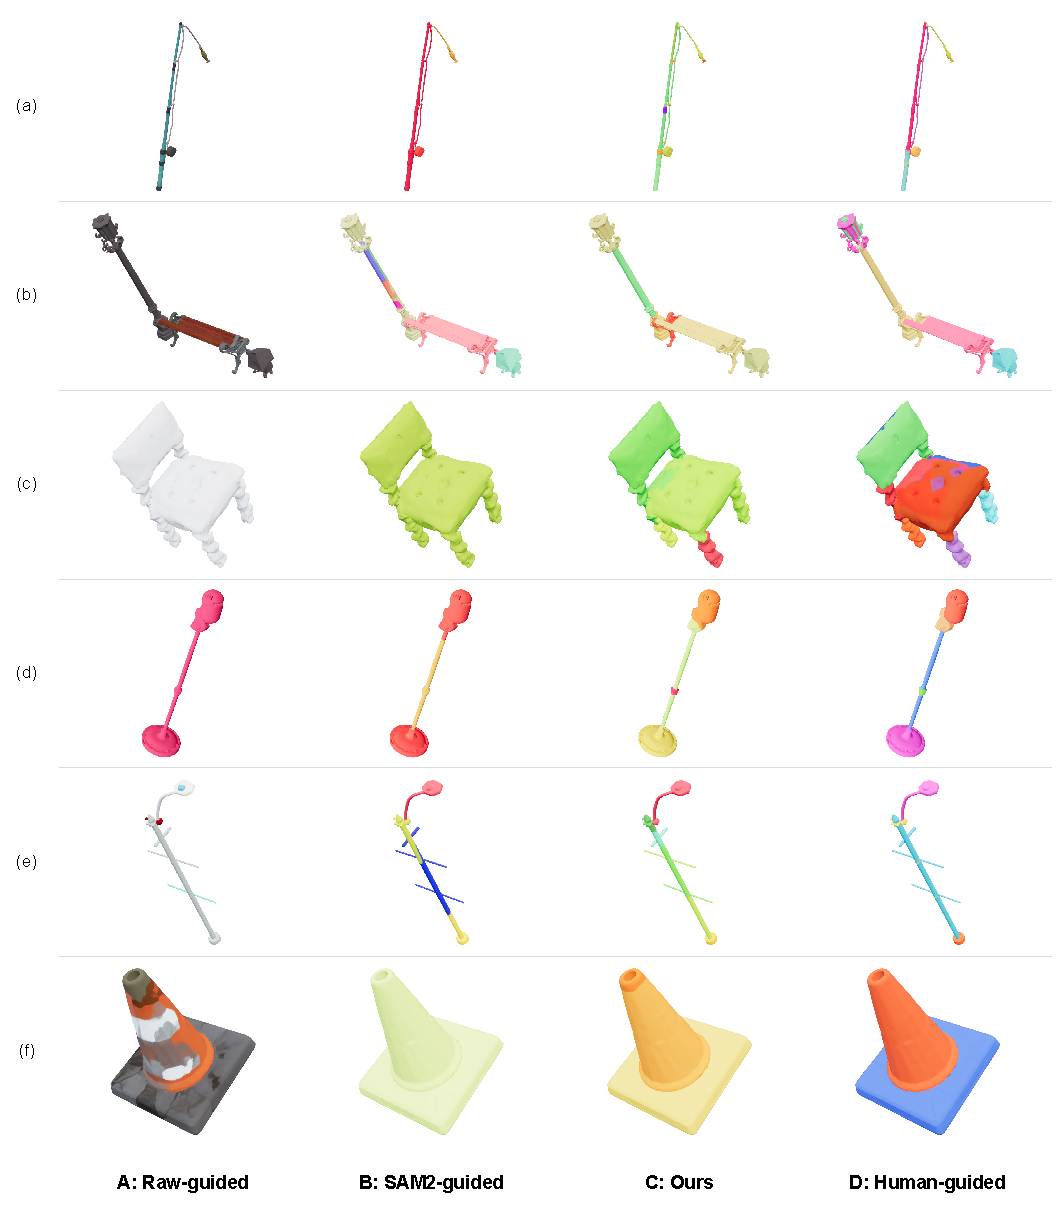
\includegraphics[width=\textwidth,height=0.80\textheight,keepaspectratio]{fig4_3d_comparison.pdf}
\caption{Final SegviGen outputs for six selected objects under A/B/C/D guidance conditions. All 24 panels are rendered from the corresponding GLB files. Columns use the raw-image condition, automatic SAM2 guidance, our assembled guidance, and human-reference guidance. Rows (a), (b), (d), and (e) are thin or fine-grained objects, row (c) is an assembly, and row (f) is a solid-volume object. Each row uses the same display view and lighting across conditions; these views are independent of the scoring cameras. Colors identify local regions within an output.}
\label{fig:qualitative}
\end{figure*}
\clearpage

\subsection{Ablation of prompting, audit, and assembly}
The ablation separates changes in prompts, audit behavior, and assembly. The planning response is held fixed wherever the component being removed does not change planning itself. Automatic SAM2 provides the image-only baseline. The box-and-point baseline runs the earlier pipeline with one positive point, no negative points, and no audit. Its assembly gives larger masks overlap priority and fills gaps through repeated $5\times5$ grayscale dilation. It does not use the proposed component cleaning, small-box priority, or distance-transform filling. This is a combined earlier-pipeline baseline, rather than a single-factor ablation of the full method.

The single-positive variant keeps the box, negative points, audit, and assembly while limiting positive support to the first point in both initial and retry calls. The no-negative variant removes negative points from both initial and corrected prompts. The no-audit variant skips all feedback calls. The no-point-filter variant bypasses both point-anchored component-filtering passes. It retains morphological closing, hole filling, area thresholds, small-box overlap priority, and distance-transform gap filling. Results are evaluated at both the 2D guidance and final-output projection levels. Table~\ref{tab:ablation} uses descriptive configuration names.

\begin{table*}[t]
\caption{Component ablation. The first three metrics evaluate the 2D guidance against the designated standard reference before 3D inference, macro-averaged over the three structural groups; evaluated pairs are 494 for Automatic SAM2, 484 for Box-And-Point, and 500 for all remaining rows. Projection mIoU evaluates the final 3D output on the 492 aligned objects and is currently available for the rows whose frozen-backend outputs exist. Each single-factor row changes the named component relative to Ours. The box-and-point baseline is the explicitly configured earlier pipeline.}
\label{tab:ablation}
\centering\small
\setlength{\tabcolsep}{5pt}
\begin{tabularx}{\textwidth}{@{}Y c c c c@{}}
\toprule
Configuration & \shortstack{2D Matched\\mIoU (\%) $\uparrow$} & \shortstack{2D BF1\\(\%) $\uparrow$} & \shortstack{2D Part F1\\at 0.5 (\%) $\uparrow$} & \shortstack{Proj. mIoU\\(\%) $\uparrow$}\\
\midrule
Automatic SAM2 & 44.80 & 44.81 & 40.36 & 35.77\\
Box-And-Point Baseline & 42.50 & 43.86 & 38.78 & \unmeasured\\
Ours With One Positive Point & 51.79 & 47.04 & 43.58 & \unmeasured\\
Ours Without Negative Points & 47.18 & 43.24 & 40.90 & \unmeasured\\
Ours Without Mask Audit & 52.11 & 47.53 & 44.20 & \unmeasured\\
Ours Without Point-Anchored Filtering & 45.46 & 40.27 & 38.93 & \unmeasured\\
Ours & 51.53 & 46.87 & 43.74 & 37.77\\
\bottomrule
\end{tabularx}
\end{table*}

Guidance and projection scores measure different stages of the pipeline. A prompt change may improve the source-view mask yet have little effect after 3D propagation. Conversely, a small boundary change may alter the grouping of an extended surface. Reporting both levels shows where an observed difference enters the pipeline. On the 500-object collection, Ours improves over Automatic SAM2 by 6.73 points in 2D matched mIoU, and over the earlier box-and-point pipeline by 9.03 points. Removing negative points reduces mIoU by 4.35 points relative to Ours, and bypassing the point-anchored component filtering reduces it by 6.07 points, identifying these two mechanisms as the largest single-factor contributions. Restricting positive support to one point or skipping the audit leaves the macro-averaged scores essentially unchanged, within 0.6 points of Ours; these components instead act on event-level robustness and the traceability of individual parts, which the projection-level measurements below complement. The ablation plot in Fig.~\ref{fig:ablationplot} remains empty until the paired uncertainty intervals are available.

\subsection{Audit feedback and correction tradeoff}
The audit trace records accepted candidates, rejected candidates, successful retries, and candidates dropped by assembly. These event counts identify which stages are active without establishing their accuracy. Accuracy changes require paired mask measurements against the reference, reported in Table~\ref{tab:audit}.

Across the collection, planning proposed 4742 parts, of which 4627 produced a valid initial mask. The audit accepted 2819 masks directly and rejected 1808, of which 716 were corrected by the single retry; five audits could not be parsed and six retries failed, in which cases the initial valid mask was retained. Assembly retained 3546 candidates and dropped 1081, and 115 proposals received no SAM2 mask at all. Feedback was triggered in 283 of the 500 objects. Replacing each rejected initial mask with its corrected retry changes the macro-averaged mIoU from 51.21 to 51.53 points, BF1 from 46.69 to 46.87, and recall from 51.06 to 51.70, a small positive mean effect associated with replacing the rejected masks. Wall-clock costs of planning and audit calls are not recorded in the retained logs and are therefore reported as unavailable.

\begin{table*}[t]
\caption{Audit feedback tradeoff on the 500 paired objects, macro-averaged with equal weight over the three structural groups. Pre-feedback assembles the first valid mask of every proposed part; post-feedback replaces each rejected mask with its single corrected retry when the retry is valid. The audit gives a small positive mean change in region agreement and recall at a bounded cost of at most one extra segmenter call per audited part; the negligible Part F1 change indicates that correction rarely alters the matched part count. Event counts: 4742 planned parts, 4627 valid initial masks, 2819 accepted directly, 716 corrected retries, five unparseable audits and six failed retries retaining the initial mask, 3546 candidates retained and 1081 dropped in assembly, and 115 proposals without a SAM2 mask; feedback was triggered in 283 of 500 objects.}
\label{tab:audit}
\centering\small
\setlength{\tabcolsep}{5pt}
\begin{tabularx}{\textwidth}{@{}Y c c c c@{}}
\toprule
Guidance Version & \shortstack{Matched mIoU\\(\%) $\uparrow$} & \shortstack{BF1\\(\%) $\uparrow$} & \shortstack{Recall at 0.5\\(\%) $\uparrow$} & \shortstack{Part F1 at 0.5\\(\%) $\uparrow$}\\
\midrule
Pre-Feedback (Initial Masks) & 51.21 & 46.69 & 51.06 & 43.77\\
Post-Feedback (One Correction) & 51.53 & 46.87 & 51.70 & 43.72\\
\midrule
Post $-$ Pre (pp) & $+0.31$ & $+0.19$ & $+0.64$ & $-0.05$\\
\bottomrule
\end{tabularx}
\end{table*}

\begin{figure*}[t]
\centering
\begin{minipage}{0.48\textwidth}\centering
\figureslot{3.0cm}{Figure 5\quad Structural-Group Results\par Measurements Pending}
\caption{Reserved for group-level guidance and projection results. A/B/C/D will use sea blue, soft blue, coral, and sea teal consistently.}
\label{fig:groups}
\end{minipage}\hfill
\begin{minipage}{0.48\textwidth}\centering
\figureslot{3.0cm}{Figure 6\quad Component Contributions\par Measurements Pending}
\caption{Reserved for paired ablation differences and uncertainty intervals computed from object-level results.}
\label{fig:ablationplot}
\end{minipage}
\end{figure*}

\subsection{Efficiency and reliability}
Timing begins at each method's required input preparation and ends at a valid final export. For our pipeline this includes planning, initial SAM2 calls, audits, retries, assembly, and SegviGen inference. Shared image-to-3D reconstruction is reported as a separate common cost. A geometry-only baseline is not charged for a stage it does not require, and any method with per-object optimization includes that computation in its total. External VLM latency is reported alongside local GPU time when the execution environment separates them. Hardware, warm-up, caching, and concurrency settings must be recorded for interpretable measurements.

Peak GPU memory uses the maximum allocated device memory over the measured inference interval, with multi-device execution reported explicitly when applicable. Runtime failure counts include invalid generation or export outcomes under a frozen validity test. The denominator is all attempted objects in the prespecified evaluation population, including attempts excluded from paired quality summaries. Successful caching events are not treated as zero-cost inference measurements. \pending{Record the hardware, repeated-timing protocol, original attempt counts, and complete measured intervals.}

Table~\ref{tab:efficiency} also reserves a collapse rate for valid exports whose partition degenerates under a declared criterion. That criterion must be fixed independently of the final scores. It cannot be inferred from the absence of a file, or equated to a small predicted part count for every object. \pending{Finalize the collapse criterion and report valid-export denominators.} Figure~\ref{fig:efficiencyplot} will show the quality-cost relation using measured values rather than illustrative bars.

\begin{table*}[t]
\caption{Efficiency and reliability under the frozen execution protocol. Runtime includes every stage required by each method after the shared reconstruction cost is separated. Memory is measured in GiB. Failure rate uses the original attempted population. Collapse rate uses valid exports under a criterion fixed before analysis. The measured failure rates count object-level generation failures over the 500-object manifest; objects held at the evaluation gate are not runtime failures. Runtime, memory, and collapse entries await clean per-object measurement.}
\label{tab:efficiency}
\centering\small
\setlength{\tabcolsep}{5pt}
\begin{tabularx}{\textwidth}{@{}Y c c c c@{}}
\toprule
Method & \shortstack{Runtime\\(s/Object) $\downarrow$} & \shortstack{Peak Memory\\(GiB) $\downarrow$} & \shortstack{Failure Rate\\(\%) $\downarrow$} & \shortstack{Collapse Rate\\(\%) $\downarrow$}\\
\midrule
Find3D \citep{ma2024find3d} & \unmeasured & \unmeasured & \unmeasured & \unmeasured\\
PartField \citep{liu2025partfield} & \unmeasured & \unmeasured & \unmeasured & \unmeasured\\
P3-SAM \citep{ma2025p3sam} & \unmeasured & \unmeasured & \unmeasured & \unmeasured\\
GeoSAM2 \citep{deng2025geosam2} & \unmeasured & \unmeasured & \unmeasured & \unmeasured\\
SegviGen \citep{li2026segvigen} & \unmeasured & \unmeasured & 0.00 & \unmeasured\\
Ours & \unmeasured & \unmeasured & 0.00 & \unmeasured\\
\bottomrule
\end{tabularx}
\end{table*}

\begin{figure}[t]
\centering
\figureslot{3.1cm}{Figure 7\quad Quality And Computational Cost\par Measurements Pending}
\caption{Reserved for measured runtime, memory, or quality-cost analysis. The same method colors will be used throughout the manuscript.}
\label{fig:efficiencyplot}
\end{figure}

\subsection{Structural-group and part-size analysis}
The three structural groups expose different interactions between proposals and region assignment. Assemblies contain neighboring components with independent identities. Solid-volume objects can be dominated by a large housing region, while thin structures offer limited pixel support and are sensitive to clipping and overlap ownership. Grouped matched mIoU, BF1, and part F1 are reported at the object level. The analysis uses the same declared annotation granularity within each object and does not interpret a larger number of predicted regions as an improvement by itself.

Supplementary Table~S1 stratifies the paired C--B difference by object part count and by reference part area. On all 500 paired objects, C exceeds B by 6.74 points in macro-averaged matched mIoU, 2.13 points in BF1, and 5.57 points in recall at IoU 0.5. The gain concentrates in medium-sized parts occupying 1--5\% of the foreground, where mIoU rises by 21.44 points, while the change on small ($\leq1\%$) parts is 2.90 points. By object part count, the gain is 8.43 points for one to five parts and 9.55 points for six to ten parts; within the eleven-or-more stratum, C is 1.56 points below B in assemblies, the one regime where the finer automatic partition retains an advantage. The complete per-stratum breakdown, including BF1 and recall for every cell, is given in the supplementary material.

\section{Conclusion}
\label{sec:conclusion}
We presented a language-guided spatial prompting pipeline for part segmentation of generated assets. The method translates visible part names into boxes and points, audits each predicted mask on the source image, and applies a single correction when needed. Deterministic assembly resolves the mask set into a foreground-complete color condition for frozen 3D propagation. Keeping the asset representation and SegviGen configuration shared isolates the effect of the guidance condition. On the 500-object aligned collection, the assembled guidance improves 2D matched mIoU by 6.74 macro-averaged points over automatic SAM2 regions, with the gain concentrated in medium-sized parts, and the improvement survives frozen 3D propagation: the final-output projection rises from 34.19\% to 37.77\% mIoU on the 492 camera-aligned objects. The component ablation identifies negative points and point-anchored component filtering as the largest single-factor contributions, while the audit loop acts as a low-cost correction with a small positive mean effect. With reference guidance, the same backend reaches 50.97\% projection mIoU, leaving a measurable gap for improving the constructed source-view partition.

\backmatter
\section*{Statements and declarations}
\subsection*{Funding}
\pending{Author funding information.}
\subsection*{Competing interests}
\pending{Author competing-interest declaration.}
\subsection*{Author contributions}
\pending{Author contribution statement.}
\subsection*{Data availability}
\pending{Release location, asset licenses, permitted redistribution, reference annotations, and evaluation manifests.}
\subsection*{Code availability}
\pending{GitHub repository URL, frozen configuration, environment, and evaluation scripts.}
\subsection*{Use of generative tools}
\pending{Authors to finalize the disclosure of AI-assisted drafting and editing and AI-edited illustrative truck assets in Fig.~\ref{fig:pipeline}. Experimental imagery and measured results must be identified separately.}

\bibliography{references}
\end{document}
